% Workshop draft.  Generic article layout: swap in the venue's style file before
% submission.  Anonymised for double-blind review: replace \repo with an
% anonymous mirror, and scrub identifying strings from the mirrored files.
\documentclass[10pt]{article}
\usepackage[margin=1in]{geometry}
\usepackage[T1]{fontenc}
\usepackage{lmodern,microtype,amsmath,amssymb,booktabs,graphicx,xcolor}
\usepackage[numbers,sort]{natbib}
\usepackage{pgfplots}\pgfplotsset{compat=1.17}
\usepackage[hidelinks]{hyperref}
\newcommand{\sstd}{s_{\mathrm{std}}}
\newcommand{\sdel}{s_{\mathrm{del}}}
\newcommand{\stime}{s_{\mathrm{time}}}
\newcommand{\repo}{\texttt{[anonymised repository]}}
\newcommand{\cond}[1]{\textsc{#1}}

\title{The Embodiment Shortcut: Action-Following Metrics\\Read the Robot, Not the Physics}
\author{Anonymous Authors}
\date{}

\begin{document}
\maketitle

\begin{abstract}
Video world models for robotics are often evaluated by \emph{action following}: an
inverse dynamics model (IDM) infers the action from generated video and is compared
with the action the generation was conditioned on. A low error is read as evidence
that the model gets the interaction right. We show that, when the action is an
actuator command, the manipulator's pose is a near-direct readout of it, and trained
IDMs read the arm and ignore the object. In a controlled MuJoCo push task with a
position-controlled arm and a pre-registered analysis, deleting the object's physics
(placing it outside every reachable push path) changes the standard metric's error by
0.15$\times$ its reference error (95\% CI [0.12, 0.19]): the object accounts for 0.3\%
of the metric's distance to chance. We propose \textbf{OG-AF} (Object-Grounded
Action-Following), which scores the frame pair at a delayed horizon after the arm has
retracted, where the object accounts for 98\%. In exploratory analyses OG-AF responds
to friction changes that shift the object's resting position by a few millimetres, while
the standard metric stays flat across a 16-fold friction range. In a separately
pre-registered world-model test, OG-AF separates a model trained on wrong physics from a
correct one with paired effect $d=1.94$ versus $0.46$ for the standard metric, whose
response is matched by its response on a no-object control.
\end{abstract}

\section{Introduction}

A video world model conditioned on a robot action should produce video in which that
action has its physical consequences \citep{yang2024unisim,bruce2024genie,nvidia2025cosmos,zhu2024irasim}.
\emph{Action following} has become a common way to check this
\citep{multiworld2026,followactions2026}: train an IDM on real video, as in VPT-style
labelling \citep{baker2022vpt}, run it on generated video, and measure how well it
recovers the conditioning action. A low error is taken as evidence that the model
follows the action, and implicitly that it gets the interaction right.

This inference fails for a structural reason. When the action is an actuator command
and the arm is position-controlled, the arm's configuration after executing the
command is close to an invertible function of it. An IDM trained to minimise
action-prediction error can recover the action from the arm alone, and the object then
carries no additional information. The metric then scores how faithfully a model
renders the robot, while being largely blind to whether contact physics was correct.
We call this the \emph{embodiment shortcut}: a shortcut in the sense of
\citet{geirhos2020shortcut}, and the evaluation-side analogue of causal confusion in
imitation learning \citep{dehaan2019causal}.

The question is not whether the arm \emph{can} carry the action (in our setup it does by
construction) but whether trained IDMs nonetheless use the object, and whether a simple
change of horizon makes the metric physics-sensitive. We find that they do not, and
that it does.

\paragraph{Contributions.}
(1)~A controlled testbed that isolates the shortcut: paired rollouts in which the
object is in the push path, out of it, or absent, with identical arm motion, and a
paired estimator (\S\ref{sec:setup}, Fig.~\ref{fig:conditions}).
(2)~Pre-registered evidence that the standard metric is insensitive to object physics
and that OG-AF is not (\S\ref{sec:confound}).
(3)~Exploratory evidence on how large a physics change each metric registers
(\S\ref{sec:resolution}).
(4)~A pre-registered world-model test in which OG-AF, but not the standard metric,
separates a model trained on wrong physics, including a diagnosed failure of our first
attempt (\S\ref{sec:wm}).

\section{Setup}
\label{sec:setup}

\begin{figure}[t]
\centering
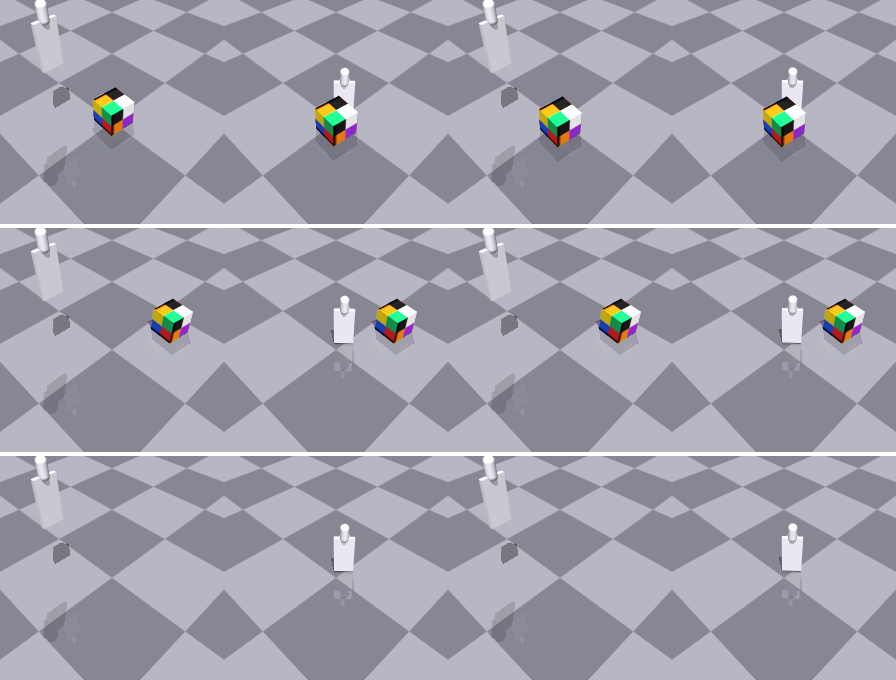
\includegraphics[width=0.9\linewidth]{figures/conditions.png}
\caption{Real renders of the three conditions for one action. Rows, top to bottom:
\cond{interact}, \cond{decoy}, \cond{absent}. Columns, left to right: $s_0$, $\sstd$,
$\sdel$, $\stime$. The arm
motion is identical in every row. At $\sstd$ the arm is mid-push and encodes the action;
at $\sdel$ it is back at rest and only the object's settled pose carries the action; at
$\stime$ the arm has not retracted.}
\label{fig:conditions}
\end{figure}

\paragraph{Task.} A 4-DOF paddle pushes one of three objects (box, sphere, cylinder)
in MuJoCo \citep{todorov2012mujoco}, rendered at $224\times224$ and 20\,fps. The action
$a=(v,\theta,d)$ (push speed 0.12--0.36\,m/s, approach angle $\pm90^\circ$, lateral
contact offset $\pm35$\,mm) is drawn uniformly. Each dimension is normalised to $[0,1]$
and we report mean absolute error over the three dimensions, for which the
uniform-prior baseline (``chance'') is 0.25. The arm is position-controlled and clamped
to the commanded path, so its motion is identical across conditions; a yaw joint makes
the map from action to arm pose invertible, the situation under study.

\paragraph{Conditions.} For each (action, seed) tuple we simulate \cond{interact} (object
in the push path), \cond{decoy} (the same object placed in an annulus verified
numerically to clear every reachable push corridor by $\geq14$\,mm, drawn from an
independent random stream so its placement carries no information about the action)
and \cond{absent} (no object). 2\,000 tuples per geometry give 18\,000 rollouts. Splits
are 80/10/10 by tuple, so paired rollouts never straddle them; the held-out set has 611
\cond{interact}/\cond{decoy} pairs after excluding rollouts that fail physics
validators (at most 1.1\% per cell).

\paragraph{Horizons} (Fig.~\ref{fig:conditions}). $\sstd$ is the last frame of the push,
the horizon the standard metric uses. $\sdel=\max(\text{object settled},\text{arm at
rest})$. $\stime$ has the same timing as $\sdel$, but the arm only withdraws by 1.5\,mm
instead of retracting, which separates retraction from elapsed time.

\paragraph{IDMs.} We follow the MultiWorld protocol \citep{multiworld2026}: a
ResNet-50 (ImageNet initialisation, our choice) with a non-causal temporal transformer,
MSE loss. \textbf{A-std} reads a 16-frame clip spanning $[s_0,\sstd]$, a faithful
reproduction of the standard metric. \textbf{A-del} (OG-AF) reads only the pair
$(s_0,\sdel)$. \textbf{A-time} reads $(s_0,\stime)$, and \textbf{A-clip-del} reads a
clip ending at $\sdel$. Each has five seeds and is trained on all three conditions, so
that no condition is out of distribution at test. Because the arm alone decodes the
action (\S\ref{sec:confound}), training on \cond{interact} only would leave the same
optimal solution available. As descriptive support we also train linear-probe-style
MLPs on frozen DINOv3 ViT-L/16 CLS features \citep{simeoni2025dinov3} (ten seeds).
DINOv3 resolves a one-frame object displacement at $+13.9\sigma$ where DINOv2
\citep{oquab2023dinov2} reaches $+0.55\sigma$.

\paragraph{Estimator.} On held-out tuples,
$G=\operatorname{mean}_p[\mathrm{err}(\cond{decoy}_p)-\mathrm{err}(\cond{interact}_p)]$,
the mean of per-pair differences. A metric that uses the object should find
\cond{decoy} much harder, giving a large $G$; one that reads only the arm gives
$G\approx0$. For a physics-sensitive metric, \emph{small $G$ is the failure}. Absolute
errors differ by $25\times$ across IDMs, so we report $G$ relative to each IDM's
reference error, its own held-out \cond{interact} error (the \cond{interact} column of
Table~\ref{tab:e}). We also report the \emph{object share},
$G/(0.25-\mathrm{err}(\cond{interact}))$: the fraction of the IDM's distance to chance
that disappears when the object's physics is removed. CIs are 95\% hierarchical
bootstrap (tuples within seeds, then seeds; 10\,000 replicates).

\paragraph{Pre-registration.} The confirmatory hypotheses, thresholds and estimators
were committed to a public repository and time-stamped (2026-09-29) before the
confirmatory experiment ran. A mechanical lock refuses to run that analysis until the
registration is public and unmodified \repo. The world-model test of \S\ref{sec:wm} was
registered separately (2026-10-05) before its corruption was calibrated or its model
trained. Thresholds were fixed at pre-declared template defaults (for example
$\tau_1=0.25$) without reference to any confirmatory statistic. A deviations log lists
every post-registration change, and none affects a confirmatory result.

\section{The standard metric ignores the object}
\label{sec:confound}

\paragraph{State oracles.} Probes on simulator state, before any pixels: arm state alone
recovers the action to 1.0--1.2\% of chance at $\sstd$, identically with and without the
object in the path. At $\sdel$ the arm carries nothing (97--98\%) while the settled
object carries 11--45\% (original 3-seed record; an independent re-run gives 0.7--0.9\%,
97--98\% and 10--48\%). The shortcut channel exists by construction. The question is
whether trained pixel IDMs use anything else.

\begin{table}[t]
\centering\small
\caption{Main experiment (held-out, pooled over geometries; 611 pairs per seed, 5
seeds). Errors as \% of chance (0.25). $G$ relative to the reference error
(= \cond{interact} column), and object share (fraction of the distance to chance removed
by deleting the object's physics). 95\% CIs.}
\label{tab:e}
\begin{tabular}{lccccc}
\toprule
IDM & \cond{interact} & \cond{decoy} & \cond{absent} & $G$ / reference & object share \\
\midrule
A-std (standard) & 1.9 & 2.2 & 1.5 & $0.15\;[0.12, 0.19]$ & 0.003 \\
A-clip-del       & 2.2 & 2.5 & 2.0 & $0.14\;[0.11, 0.16]$ & 0.003 \\
A-time           & 4.1 & 4.2 & 3.2 & $0.02\;[-0.01, 0.06]$ & 0.001 \\
\textbf{A-del (OG-AF)} & \textbf{44.7} & \textbf{99.0} & 98.5 & $\mathbf{1.21\;[1.18, 1.24]}$ & \textbf{0.98} \\
\bottomrule
\end{tabular}
\end{table}

\paragraph{Confirmatory test 1: insensitivity of the standard metric.} Deleting the
object's physics raises A-std's error by $0.15\times$ its reference error, below the
pre-registered threshold $\tau_1=0.25$ (CI upper bound 0.19; Holm-adjusted one-sided
$p\leq0.0002$, the bootstrap's resolution). The gap is above zero, so the IDM uses the
object slightly, but the object accounts for only 0.3\% of A-std's distance to chance.
A-std is also \emph{better} with no object at all (1.5\% versus 1.9\%), consistent with
the object occluding or distracting from the arm.

\paragraph{Confirmatory test 2: OG-AF reads the object.} At $\sdel$ OG-AF recovers the
action from the settled object at 44.7\% of chance (Holm $p\leq0.0002$). As registered,
this test is close to automatic, because it reduces to ``better than chance''. The
informative number is the contrast with \cond{decoy}, where OG-AF is at chance (99.0\%),
as it must be: at $\sdel$ the arm is at rest in every condition. The object share is
0.98.

\paragraph{Descriptive checks.} \emph{Retraction, not elapsed time:} A-time behaves like
A-std ($|\Delta G|=0.0005$ in normalised error) and not A-del (0.135), so the effect
comes from the arm retracting. \emph{Clip access:} an IDM given a clip that ends at
$\sdel$ (A-clip-del) re-opens the shortcut, with $G$ matching A-std, so OG-AF must score a
frame pair, not a clip. The frozen-feature probes show the same pattern ($G\approx0$ at
$\sstd$, large at $\sdel$).

\section{How large a physics change each metric registers (exploratory)}
\label{sec:resolution}

\begin{figure}[t]
\centering
\begin{minipage}{0.49\linewidth}% GENERATED by scripts/paper_figures.py from results/ -- do not edit
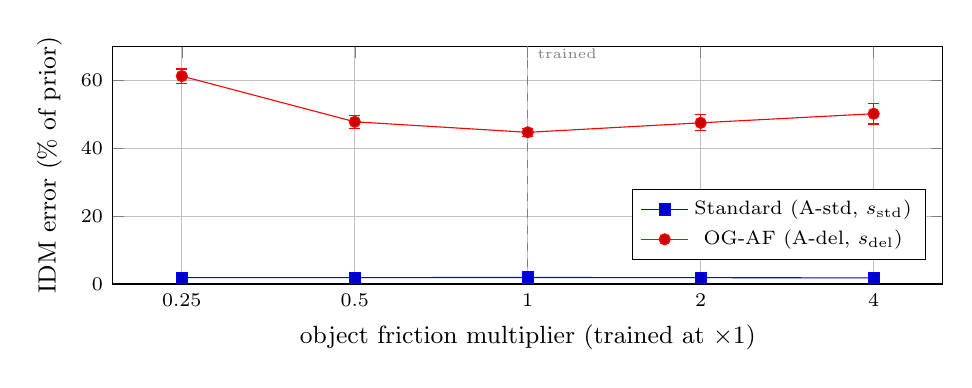
\begin{tikzpicture}\begin{axis}[width=\linewidth, height=4.6cm, xmode=log, log basis x=2,
  xlabel={object friction multiplier (trained at $\times1$)}, ylabel={IDM error (\% of prior)},
  xtick={0.25,0.5,1,2,4}, xticklabels={0.25,0.5,1,2,4}, ymin=0, ymax=70, grid=major,
  legend style={font=\scriptsize, at={(0.98,0.10)}, anchor=south east}, tick label style={font=\scriptsize},
  label style={font=\small}]
\draw[gray, dashed] (axis cs:1,0) -- (axis cs:1,70) node[pos=0.97, right, font=\tiny] {trained};
\addplot+[blue, mark=square*, error bars/.cd, y dir=both, y explicit] coordinates {(0.25,1.89541) +- (0,0.0934484) (0.5,1.89706) +- (0,0.0954691) (1,1.92642) +- (0,0.0554075) (2,1.88275) +- (0,0.119297) (4,1.80327) +- (0,0.126877)};
\addlegendentry{Standard (A-std, $s_\mathrm{std}$)}
\addplot+[red, mark=*, error bars/.cd, y dir=both, y explicit] coordinates {(0.25,61.2471) +- (0,2.07702) (0.5,47.7875) +- (0,1.92464) (1,44.6862) +- (0,1.15089) (2,47.4878) +- (0,2.33843) (4,50.1627) +- (0,3.02961)};
\addlegendentry{OG-AF (A-del, $s_\mathrm{del}$)}
\end{axis}\end{tikzpicture}
\end{minipage}\hfill
\begin{minipage}{0.49\linewidth}% GENERATED by scripts/paper_figures.py from results/ -- do not edit
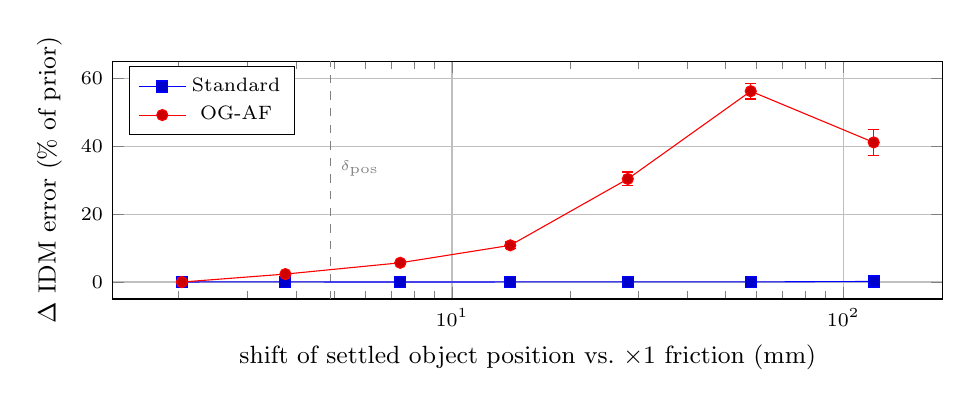
\begin{tikzpicture}\begin{axis}[width=\linewidth, height=4.6cm, xmode=log,
  xlabel={shift of settled object position vs.\ $\times1$ friction (mm)},
  ylabel={$\Delta$ IDM error (\% of prior)}, grid=major, ymin=-5, ymax=65,
  legend style={font=\scriptsize, at={(0.02,0.98)}, anchor=north west}, tick label style={font=\scriptsize},
  label style={font=\small}]
\draw[gray, dashed] (axis cs:4.9,-5) -- (axis cs:4.9,65) node[pos=0.55, right, font=\tiny] {$\delta_{\mathrm{pos}}$};
\addplot+[blue, mark=square*, error bars/.cd, y dir=both, y explicit] coordinates {(2.0398,0.0122332) +- (0,0.0628719) (3.75225,0.0272257) +- (0,0.0431282) (7.37503,-0.00958196) +- (0,0.0374989) (14.0888,0.0187233) +- (0,0.0406763) (28.134,0.0406467) +- (0,0.0623473) (57.9979,0.0211003) +- (0,0.0669174) (119.551,0.149998) +- (0,0.0773357)};
\addlegendentry{Standard}
\addplot+[red, mark=*, error bars/.cd, y dir=both, y explicit] coordinates {(2.0398,-0.0128842) +- (0,1.22473) (3.75225,2.33089) +- (0,0.502062) (7.37503,5.654) +- (0,0.628609) (14.0888,10.8011) +- (0,0.975772) (28.134,30.356) +- (0,2.03855) (57.9979,56.1944) +- (0,2.29602) (119.551,41.1147) +- (0,3.78085)};
\addlegendentry{OG-AF}
\end{axis}\end{tikzpicture}
\end{minipage}
\caption{\textbf{Left:} IDMs trained at friction $\times1$, scored on held-out rollouts
with changed object friction (95\% CI). The standard metric stays at 1.8--1.9\% while
the object comes to rest up to 6\,cm away; OG-AF rises on both sides of the training
value. \textbf{Right:} change in IDM error (percentage points of chance) against the
physics-induced shift of the object's resting position, binned. 1\,570
(tuple, friction) pairs over friction $\times\{0.1,0.25,0.5,2,3,4\}$;
$\delta_{\mathrm{pos}}=4.9$\,mm is the 5th-percentile per-frame object displacement.}
\label{fig:resolution}
\end{figure}

Neither analysis in this section was pre-registered as a confirmatory test.

\paragraph{Friction sweep.} We score the trained IDMs on rollouts whose object friction
is changed from $\times0.25$ to $\times4$ (Fig.~\ref{fig:resolution}, left). The arm is
identical across frictions, so the standard metric stays at 1.8--1.9\% of chance,
although the object comes to rest up to 6\,cm away (median 20\,mm at $\times0.25$).
OG-AF's error rises away from the training friction in both directions: 61.2\% at
$\times0.25$ and 50.2\% at $\times4$, versus 44.7\% at $\times1$. The differences at
$\times0.5$ and $\times2$ are small. A prediction of a \emph{monotone} response, in our
protocol specification, was mis-specified for an IDM trained at $\times1$, and is
reported as failed.

\paragraph{Error change versus displacement.} For each held-out tuple and friction
level we pair the simulator's shift of the object's resting position with the change in
each IDM's error (Fig.~\ref{fig:resolution}, right). On the friction levels of the sweep
alone, OG-AF's error rises significantly from the 2.5--5\,mm bin on
($+2.1$ points, 95\% CI $[+1.4,+2.9]$), and the standard metric shows no significant
change in any bin up to 40\,mm. Adding the $\times0.1$ and $\times3$ corpora built for
\S\ref{sec:wm} extends the range: OG-AF's paired effect grows from $d=0.64$ at
2.5--5\,mm to 3.27 at 40--80\,mm. The standard metric's only nonzero response,
$+0.15$ points, appears beyond 80\,mm and comes entirely from $\times0.1$ rollouts.
OG-AF's response drops beyond 80\,mm, plausibly as resting positions leave the range seen
in training.

This flatness is a property of the design as much as of the metric: in a
position-controlled setup, physics cannot move the arm, and the standard metric reads
the arm. OG-AF's reference error is higher (44.7\% versus 1.9\% of chance). It gives up
precision on the action to gain sensitivity to the interaction, which is what an
action-following metric is meant to measure.

\section{World models: catching wrong physics}
\label{sec:wm}

\paragraph{Models.} We train factorised spatio-temporal video transformers (90.5M
parameters) over the $4\times28\times28$ latents of a compact convolutional VAE, with
AdaLN action conditioning and strict temporal causality. Each is trained for 120k steps
on \cond{interact} clips of all three geometries, 16 frames spanning $[s_0,\sdel]$. Each
model generates the 193 held-out box tuples deterministically and autoregressively from
the real first frame. The registered ladder has WM-base at 100\%, 30\% and 10\% of its
training steps, a model trained on 10\% of the data, and a model trained on wrong
physics. Generated video is scored with IDMs trained with mild appearance augmentation
(colour jitter, blur, compression artefacts; seed 0). Real-video numbers elsewhere use
unaugmented IDMs averaged over five seeds.

\paragraph{Ranking agreement.} On every model the standard and OG-AF metrics rank the
same generated rollouts almost independently (Spearman $\rho\leq0.28$). This is
descriptive: the $<0.9$ criterion in our analysis code is lax and does not appear in the
registration.

\paragraph{A diagnosed failure.} Our first ladder failed its validity check: models were
not monotone in ground-truth error (Spearman 0.70, below the 0.9 our analysis requires),
which voided the between-model claim as registered. The check measured whole-frame pixel
error, which is dominated by how the arm and background are rendered (the object covers
roughly 2\% of the frame). The corruption (friction $\times3$) was also never checked to
be large. The validity check fell for the very shortcut it was meant to guard against.

\paragraph{The registered fix.} Before running anything, we registered a second ladder.
Its ground truth is object-region error: pixels where the real \cond{interact} and
\cond{absent} frames differ. Its corruption is chosen mechanically from friction
$\times\{0.1,0.25,4,10\}$ as the mildest candidate whose \emph{real} video already
differs from correct physics by at least $1.25\times$ the weakest correct model's
object-region error, with at least 80\% of rollouts passing the physics validators.
Only $\times0.1$ qualified. By intent, this makes the corrupted model's position at the
bottom of the ladder likely; whether models 1--4 are ordered correctly is not
constrained.

\begin{figure}[t]
\centering
\begin{minipage}{0.5\linewidth}% GENERATED by scripts/paper_figures.py from results/ -- do not edit
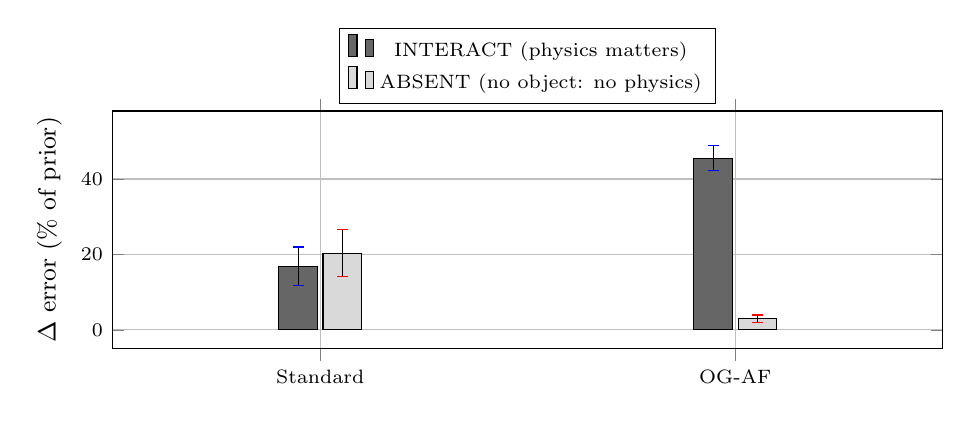
\begin{tikzpicture}\begin{axis}[width=\linewidth, height=4.6cm, ybar, bar width=14pt,
  symbolic x coords={Standard,OG-AF}, xtick=data, enlarge x limits=0.5, ymin=-5, ymax=58,
  ylabel={$\Delta$ error (\% of prior)}, grid=major,
  legend columns=1,
  legend style={font=\scriptsize, at={(0.5,1.03)}, anchor=south},
  tick label style={font=\scriptsize}, label style={font=\small}]
\addplot+[fill=black!60, draw=black, error bars/.cd, y dir=both, y explicit] coordinates {(Standard,16.898) +- (0,5.051) (OG-AF,45.488) +- (0,3.273)};\addlegendentry{INTERACT (physics matters)}
\addplot+[fill=black!15, draw=black, error bars/.cd, y dir=both, y explicit] coordinates {(Standard,20.277) +- (0,6.216) (OG-AF,2.924) +- (0,1.009)};\addlegendentry{ABSENT (no object: no physics)}
\end{axis}\end{tikzpicture}
\end{minipage}\hfill
\begin{minipage}{0.47\linewidth}\small
\caption{Change in mean IDM error, wrong-physics world model (friction $\times0.1$)
minus correct WM-base, on the same 193 held-out tuples, in percentage points of chance
(95\% paired-bootstrap CIs). The standard metric rises as much on \cond{absent}, where
there is no object and physics cannot matter, as on \cond{interact} (difference
$-3.4$ points, CI $[-8.3,+1.2]$). OG-AF rises by 45.5 points on \cond{interact} and
2.9 on \cond{absent}.}
\label{fig:h2}
\end{minipage}
\end{figure}

\paragraph{Confirmatory test 3: the wrong-physics model.} The rebuilt ladder is
monotone in object-region error (Spearman 1.00; 0.057, 0.059, 0.070, 0.114, 0.162).
Paired over the same tuples, the wrong-physics model differs from the correct one by
$d=1.94$ [1.73, 2.22] under OG-AF and $d=0.46$ [0.37, 0.56] under the standard metric.
The registered contrast is $\Delta d=1.48$ [1.22, 1.79], which supports the
hypothesis. The standard metric does respond, but its response is no larger on
\cond{interact} than on the no-object control (Fig.~\ref{fig:h2}). This is consistent
with a rendering difference and not a physics one; the corrupted model also lost 12.6\%
of its training rollouts to the physics validators. For OG-AF, the difference between the
\cond{interact} and \cond{absent} responses is $+42.6$ points [38.8, 46.1]. The corruption is gross: OG-AF scores the
model near chance (92.4\%).

\paragraph{Domain gap.} On generated video the standard metric's error is 56--57\% of
chance for the base models (1.9\% on real video), and 61--64\% on the \cond{absent}
control. On generated video it largely measures rendering fidelity. OG-AF sits near its
real-video reference (47\% versus 44.7\%) and near chance on \cond{absent}. Part of this
robustness is structural: half of OG-AF's input is the real conditioning frame, and the
arm at rest is easy to render. These numbers come from small self-trained models and may
not transfer to larger ones.

\section{Related work}
Action-conditioned video world models for robotics
\citep{yang2024unisim,du2023unipi,bruce2024genie,nvidia2025cosmos,zhu2024irasim} are
increasingly evaluated by action following with IDMs \citep{multiworld2026}, building on
IDM-based action labelling \citep{baker2022vpt,ye2024lapa}. A recent diagnosis of whether
robotic world models follow actions measures end-effector trajectories, i.e.\ arm
kinematics, by design \citep{followactions2026}. A position paper argues that
decision-relevant evaluation, not visual fidelity, should guide world-model assessment
\citep{pipeline2026}. Physical-plausibility benchmarks evaluate generated video directly
\citep{bear2021physion,kang2024phyworld,bansal2024videophy,motamed2025physicsiq}; we
study an evaluation pipeline already in use. The World Action Verifier \citep{wav2026}
assumes a verification subset whose next state depends only on its own state and the
action, and proves that a sparse inverse model transfers under that assumption. Read as
an evaluation metric, the condition is object-blindness: in our data it holds at $\sstd$
and fails at $\sdel$. The guarantee and the confound are the same property used for
different purposes. More broadly, the embodiment shortcut is an instance of shortcut
learning \citep{geirhos2020shortcut,lapuschkin2019cleverhans} and of causal confusion
\citep{dehaan2019causal}.

\section{Limitations}
\textbf{Scope.} Simulation only: one push task, three primitive objects, a
position-controlled arm whose trajectory contact cannot perturb, and small world models
trained on their own corpus. On compliant or torque-controlled arms, contact perturbs
the arm, so the arm channel will carry some physics signal, entangled with embodiment.
The shortcut should shrink there but not vanish. Transfer to real robot data and to
published world models is the main open question.
\par\textbf{Generality of OG-AF.} OG-AF needs a horizon at which the manipulator is at rest
and the object has settled, which suits primitive-level actions. High-rate continuous
control, grasping in which the arm stays in contact, and multi-step tasks would need
extensions such as scoring at action-chunk boundaries, masking or inpainting the arm,
or object tracking. Because OG-AF sees only the end state, it cannot detect wrong
intermediate dynamics that end in the right state. Masking the arm at $\sstd$ is a
natural alternative: in our frozen-feature probes, object pixels alone reach 48\% of
chance at $\sstd$. Directly comparing tracked object trajectories with paired real
video is another, where such video exists.
\par\textbf{World-model evidence.} One corruption type, which is gross; one IDM seed;
193 held-out box tuples (the registration anticipated 1\,500, but the test split holds
193). The wrong-physics corpus lost 8--18\% of rollouts per geometry to the physics
validators, so that model also saw less data.
\par\textbf{Other.} DINO features are blind to sub-degree rotation. The analyses of
\S\ref{sec:resolution} are exploratory. Two exploratory predictions failed as worded,
the friction monotonicity and the orderings of a pixel-masking decomposition, and are
reported as such.

\section{Conclusion}
Action following, as practised, rewards rendering the robot correctly. Scoring at a
horizon where the manipulator no longer encodes the action turns the same pipeline into
a measurement of the interaction. We recommend that action-following results report an
object-grounded variant and a no-object control alongside the standard number.

\paragraph{Reproducibility.} Code, both registration documents, the deviations log,
every result record, and the generators for all tables and figures are in \repo. One
command resubmits the pipeline on a SLURM cluster. The full study used roughly 80
GPU-hours (A100/L40S), plus older GPUs for rendering.

\paragraph{Use of AI assistance.} An AI coding agent (a large language model)
implemented and audited substantial parts of the pipeline and analysis code, drafted
parts of the manuscript, and, at the researchers' delegation, fixed the open
registration values: the template defaults, and the design of the world-model
registration. It did so before any confirmatory statistic existed, as recorded in both
registration documents. The researchers reviewed the code, analyses and text and take
responsibility for all decisions and claims.

\small
\bibliographystyle{plainnat}
\bibliography{refs}
\end{document}
